\section{Имплементация}
\begin{Large}
За изобразяване на фрактала е направена имплементация на C++, използваща главно стандартни библиотеки и дефинирането на структура RGB, пазеща по един байт съответно за червен, зелен и син цвят на пиксела. Избраният формат на изображението е PPM - това е тип bitmap, с прост и кратък header. Изображението се запазва ред по ред, започвайки от най-горния, като в използвания тип P6, файлът е в двоичен запис. Програмата работи по следният начин:
 \begin{enumerate}
\item Попълват се дадените стойности по подразбиране в новосъздадени променливи.
\item Приемат се стойности на съответните командни параметри, ако са зададени.
\item Създават се масив за нишките и указател към двумерен масив от RGB.
\item Main пуска максималния брой нишки, след което изчаква завършването им.
\item Нишките правят изчисления по "линейния метод" \ от предната глава и сами попълват информация в RGB масива всеки път щом приключат с итерирането за съответния пиксел.
\item Main създава PPM файла, попълва заглавната му част, а след това записва информацията от попълнения масив с RGB стойности.
\item Терминация 
 
 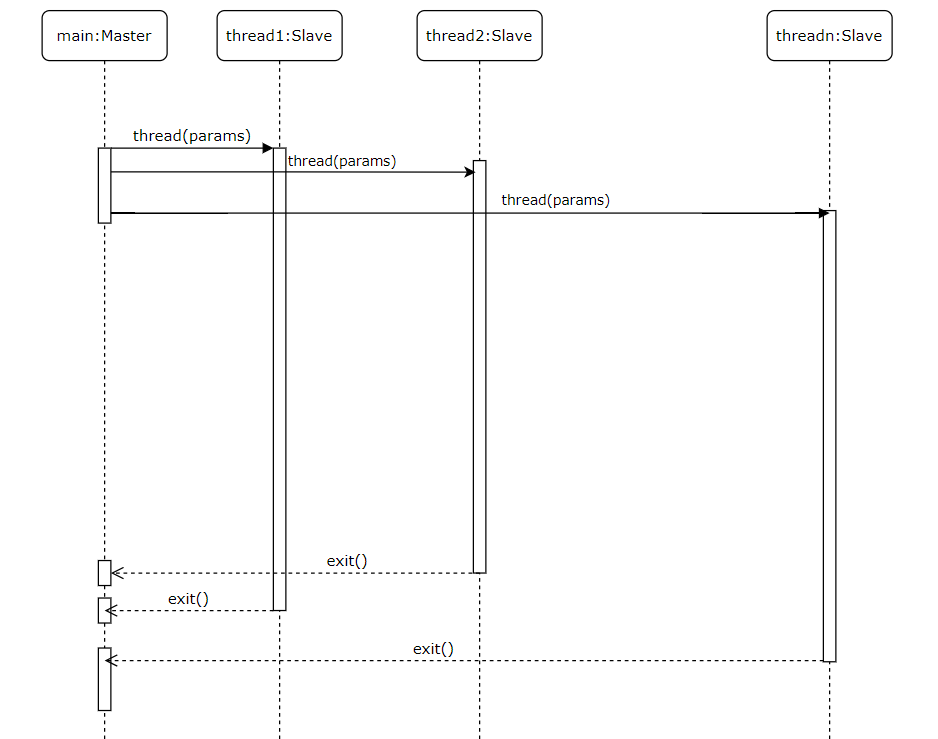
\includegraphics[width=14cm,height=12cm]{SequenceDiagram}
 
 Понеже не бе намерено достатъчно условие, което да поставим в цикъла за пикселите, е поставено следното чисто евристично условие: Ако за някоя итерация $z_n$ напусне кръга, определен от описаната около правоълълната област окръжност(т.е. при $\left\Vert z_n -\frac{(x_{min}+x_{max})+(y_{min}+y_{max})i}{2}\right\Vert > \frac{\sqrt{(x_{max}-x_{min})^2+(y_{max}-y_{min})^2}}{2}$ , то ще приключваме итерирането. Друго възможно условие би било например да се разглежда разстоянието м/у $c$ и $z_n$. 
 
 \end{enumerate}

\end{Large}
 